% $Id: circuit.tex 5679 2017-10-13 15:24:08Z mskala $

%
% MSK 010 circuit explanation
% Copyright (C) 2017  Matthew Skala
%
% This program is free software: you can redistribute it and/or modify
% it under the terms of the GNU General Public License as published by
% the Free Software Foundation, version 3.
%
% This program is distributed in the hope that it will be useful,
% but WITHOUT ANY WARRANTY; without even the implied warranty of
% MERCHANTABILITY or FITNESS FOR A PARTICULAR PURPOSE.  See the
% GNU General Public License for more details.
%
% You should have received a copy of the GNU General Public License
% along with this program.  If not, see <http://www.gnu.org/licenses/>.
%
% Matthew Skala
% https://northcoastsynthesis.com/
% mskala@northcoastsynthesis.com
%

\chapter{Circuit explanation}

\section{Reference voltage generator}

At the heart of the MSK~008's quantizer circuit, the section shown in
Figure~\ref{fig:vgen} generates six reference voltages:  $\pm$4.50V,
$\pm$1.50V, and $\pm$0.50V.  This section is shared between the two channels
in the module.

\begin{figure}
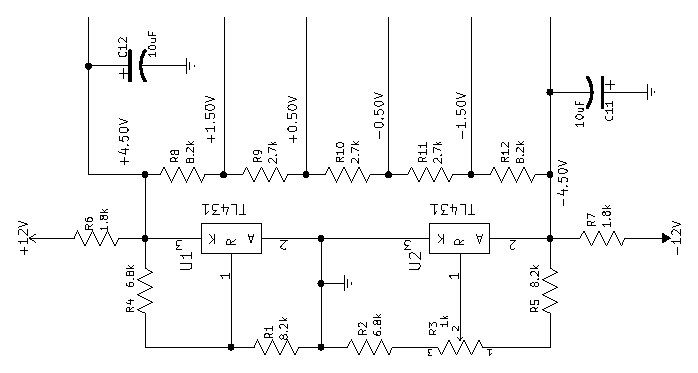
\includegraphics[angle=-90]{vgen.eps}
\caption{The voltage generator section.}\label{fig:vgen}
\end{figure}

The voltages shown in Figure~\ref{fig:vgen} are nominal values only.  The
actual voltages of these references will vary because of component
tolerances, and even the $-$4.50V reference, which can be adjusted more or
less directly by R3, may actually end up adjusted to a voltage not exactly
$-$4.50V in order to help compensate for inaccuracies elsewhere in the
module.  The function of these references is primarily to be stable, and
close enough to the nominal values to allow the rest of the circuit to work
correctly, rather than for them to be specific accurate voltages.  For this
reason, it's not necessary to use a close-tolerance version of the TL431
regulator; the default standard version (which might be 2\%\ tolerance) is
fine.

The first thing to understand in analysing this circuit is the function of
the TL431.  This IC has a fairly complicated circuit inside it, but to the
outside world it appears relatively simple.  It's a shunt voltage regulator,
used very much like a Zener diode.  In fact, some versions of the circuit
symbol depict it as a Zener diode with an extra pin, and the letters ``K''
and ``A'' in the diagram, for ``cathode'' and ``anode,'' reflect the
Zener-diode analogy.  The critical difference is that it also has that third
pin, labelled ``R'' for ``reference.''

When operating normally in a circuit that allows it to do so, the TL431 will
pass whatever current from cathode to anode is necessary to keep the
reference pin 2.495V above the anode.  If you connected the reference pin
and cathode directly together, it would be just like a 2.495V Zener diode
with unusually good temperature stability and turn-on characteristics.  But
here we are driving the reference pin from the cathode through a voltage
divider.  In the case of U1, the divider is R1 and R4, and the voltage on
the reference pin is
$8.2\textrm{k}\Omega/(6.8\textrm{k}\Omega+8.2\textrm{k}\Omega)=0.5467$ times
the voltage on the cathode.  Then in order for the reference voltage to be
2.495V, the voltage on the cathode needs to be 4.564V\@.  The TL431, if it
can, will draw enough current through its cathode to make that true.  By
adding the voltage divider, we have in effect programmed U1 to behave like a
4.564V Zener diode.  Tolerance variation in any of the three components may
push this voltage off by a few percent in either direction.

In the case of U2, there is the 1k$\Omega$ potentiometer R3 inserted into the
middle of the voltage divider to make the ratio adjustable, but it's
otherwise the same circuit, and we'd normally expect that pot to be adjusted
to roughly the same ratio as in the U1 circuit; the nominal $-$4.50V reference
will be close to the negative of the nominal 4.50V reference.

Like a Zener diode, the TL431 only works well over a specified range of
shunt currents.  That's partly because it needs a source of energy for its
complicated internal circuit (error amplifier, precision reference, and so
on).  Since it functions as a sort of amplifier with feedback, there may
also be a concern about stability:  when the load is capacitive and within a
certain range, a TL431 may go into parasitic oscillation.  So we need to
ensure that the chips stay within the operating range where they can work
normally, and that is accomplished by R6, R7, C11, and C12.

If the cathode of U1 is at about 4.50V, and the positive power supply is
about 12V, then we have about 7.5V across R6, resulting in a current of
4.167mA.  Out of that, we must subtract about 367$\mu$A for the resistor
chain R8\ldots R12, another 300$\mu$A for the voltage divider driving the
TL431 reference input, and whatever current is drawn by the other parts of
the circuit that use this reference.  That is up to 45$\mu$A for the 4.50V
reference (because it drives two adjustable resistances each at least
200k$\Omega$ into virtual ground).  For the $-$4.50V reference the other parts
of the circuit actually draw current (worst-case about 1mA of it) into
negative supply instead of into ground, with the effect of increasing the
current through U2 and making the regulator's job even easier.  The net
current through each regulator stays between about 3.5mA and 5.0mA, which is
comfortably within their advertised operating range of 1mA to 100mA.

As for stability, the 10$\mu$F capacitors, in parallel with whatever other
capacitances may exist in the circuit, ensure that each regulator sees an
effective capacitance of at least 10$\mu$F, placing it safely out of the
danger zone which for these circuit parameters would be from around
0.01$\mu$F to 2$\mu$F.  This technique could still fail in case of a really
badly behaved load that acts like an inductor and cancels out part of the
capacitance, but there is nothing like that in the actual circuit that uses
these reference voltages.  In fact, the stray capacitance that does exist is
probably small enough that we would probably be safe on the other side of
the danger zone without C11 and C12; they are included out of an abundance
of caution and to help filter out any high-frequency garbage that might get
into the reference busses from other sources.

Given the $\pm$4.50V references, the remaining reference voltages are
generated by a straightforward resistor chain, R8\ldots R12.  For perfectly
correct ratios the 8.2k$\Omega$ resistors ought to be exactly three times
the 2.7k$\Omega$ resistors (thus 8.1k$\Omega$), and that is not quite true,
but it's close enough.  If you do a more precise calculation, you may
note that the error from using 8.2k$\Omega$ resistors here is in the
opposite direction from, and will to some extent cancel out, the earlier error
of the $\pm$4.50V references being really more like $\pm$4.564V.  However,
that fortunate cancellation is something of an illusion, because the
component tolerances are not precise enough to really say anything more than
``close enough.'' The $\pm$4.50V references can each source or sink more
than 1mA without challenging the regulators; the $\pm$1.50V and $\pm$0.50V
references cannot handle so much without being pulled off voltage, but
they drive only the very-high-impedance inputs of LM339 chips with bias
currents measured in nA.

\section{Manual octave switch}

The QUA input jacks go into resistor voltage dividers like this one:

{\centering\input{manual-switch.tex}\par}

This is a passive mixer intended to add or subtract about 1V from the input
under control of the three-position toggle switch; it's not very accurate
but produces results that are close enough given we only really care about
the positions of the four quantizer rounding boundaries, which are $\pm$0.5V
and $\pm$1.5V.  The input jack connects to $V_\textrm{in}$ and the toggle
switch either is an open circuit (centre position) or connects the node
labelled SW to one of the power rails, which (taking into account a nominal
drop of 0.2V for the Schottky protection diodes) are $\pm$11.8V.  The
quantizer will switch states when $V_\textrm{q}$ crosses the $\pm$0.5V and
$\pm$1.5V boundaries.  From these known voltages it's straightforward to
apply Ohm's and Kirchhoff's Laws to find the values for $V_\textrm{in}$ to
bring $V_\textrm{q}$ to each of these boundaries in each state of the
switch.

\vspace{\baselineskip}

\begin{tabular}{c|c|c}
  \multicolumn{3}{c}{switch state} \\
  $-$1 & 0 & $+$1\\ \hline
  $+$2.50V & $+$1.50V & $+$0.73V \\
  $+$1.42V & $+$0.50V & $-$0.35V \\
  $+$0.35V & $-$0.50V & $-$1.42V \\
  $-$0.73V & $-$1.50V & $-$2.50V \\
  \multicolumn{3}{c}{\quad}
\end{tabular}
\begin{tabular}{r}
  bin \\
  \quad \\
  \raisebox{1.6ex}[0pt][0pt]{\}$+$2V} \\
  \raisebox{1.6ex}[0pt][0pt]{\}$+$1V} \\
  \raisebox{1.6ex}[0pt][0pt]{\}$\phantom{+}$0V} \\
  \raisebox{1.6ex}[0pt][0pt]{\}$-$1V} \\
  \raisebox{1.6ex}[0pt][0pt]{\}$-$2V}
\end{tabular}

Note that the boundaries shift in the opposite direction from the switch:
to have the effect of adding 1V to the input, we \emph{subtract}
approximately 1V from the quantizer boundaries, so the same input will fall
into a bin 1V higher.

As an intuition for where the design came from, consider that if we just
connected $V_\textrm{in}$ to $V_\textrm{q}$ with a 75K$\Omega$ resistor, we
could shift the voltage at $V_\textrm{q}$ up or down perfectly by 1V by
adding or subtracting a $1\textrm{V}/75\textrm{k}\Omega=13.33\mu\textrm{A}$
current at the $V_\textrm{q}$ node.  A true constant-current source would be
more complicated to build, but a high voltage applied through a high
resistance is a way of faking it.  Then the $\pm$11.8V power supply rails,
applied through 1M$\Omega$, look approximately like a $\pm$11.8$\mu$A
current source (exact only when $V_\textrm{q}$ is at 0V), which is close
enough.  The resistor values were chosen by choosing R15 to be 1M$\Omega$ as
a convenient high resistance, and then running the calculation backwards and
choosing a nearby standard value to get 75k$\Omega$ for R14.

\section{Quantizer building blocks}

The first thing to understand in the quantizer circuit is the basic function
of the LM339 comparator.  Its symbol looks like an op amp symbol, and much
of its internal circuitry resembles that of an op amp.

{\centering\input{comparator.tex}\par}

Comparators are optimized for different parameters compared to op amps, but
the most important difference between the LM339 in particular and a standard
op amp is in its output.  Instead of giving its output as a voltage or as a
current, the LM339 presents an \emph{output impedance} that depends on the
difference between its inputs.  If the positive input is at a higher
voltage, the output is high-impedance, looking like an open circuit.  If the
negative input is at a higher voltage, then the output is low-impedance,
looking like a short circuit into the negative power supply, both conditions
only being true in the ideal and approximated up to the limits of the
chip's capabilities.

This kind of output is implemented using an NPN
transistor with its collector pointing at the output pin and no pull-up
circuitry, so it's called an \emph{open collector} output.  (\emph{Open
drain} for a similar kind of output implemented with a MOSFET.)  They're
commonly used for devices like comparators which might be applied at the
interfaces between systems with different power supplies, because one can
attach an external pull-up circuit referenced to a different power
supply from the comparator's own power and get conversion between the
different voltage standards at very little cost.

Here, we're going to use an external pull-up circuit to massage the output
into a format that will be useful by the output summing amplifier and LED
driver circuits.  A section of the following form occurs in four places in
the MSK~008.

{\centering\input{comp-curr.tex}\par}

The node labelled $I_\textrm{out}$ is the virtual-ground summing node of the
output amplifier, which will be discussed later.  It is held at a constant
potential of 0V while other sections apply different currents to it.  The
$+$1.50V and $-$4.50V voltages come from the reference-voltage generator. 
And $V_\textrm{q}$ is the quantizer input voltage that comes from the QUA
jack with a possible adjustment for the manual octave switch.

When $V_\textrm{q}$ is less than the $+$1.50V reference voltage, the
output of the comparator looks like an open circuit.  Then R18 is out of the
circuit, and the diode is reverse-biased, so it also looks like an open
circuit, and R28 is also taken out.  No current, or only a very small
leakage current, flows.

But when $V_\textrm{q}$ exceeds $+$1.50V, the comparator turns on.  Its
output voltage drops to about $-$11.6V; that is the $-$11.8V power supply
voltage plus about 0.2V consumed by the saturated output transistor. 
Remembering that the $I_\textrm{out}$ node is held at 0V, the voltage
divider of R18 and R28 will try to bring the diode's cathode to a
voltage of about $-$10.6V.  But the diode is now forward biased, so it will
conduct as much current from the $-$4.50V bus as necessary to prevent its
forward voltage from growing too large.  Suppose the diode's forward voltage
is 0.49V.  Then the diode's cathode will be at $-$4.99V; and then the
current sunk through the circuit output is exactly 10$\mu$A by
Ohm's Law on R28.

So the overall action of this section is that it sinks a tightly controlled
amount of current through $I_\textrm{out}$: either 10$\mu$A when
$V_\textrm{q}$ exceeds $+$1.50V, or zero when $V_\textrm{q}$ does not exceed
$+$1.50V.  The forward voltage of D1 under these conditions is probably not
really 0.49V, but we can correct for that, assuming all the diodes in the
different instances of this section are reasonably similar to each other, by
fudging the value of the $-$4.50V reference.  Recall that the circuit which
supplies that bus includes the trimmer R3 for this purpose.

Another very similar section also occurs in four places in
the MSK~008; it differs by the addition of two more diodes.

{\centering\small\input{comp-curr2.tex}\par}

When $V_\textrm{q}$ is less than the reference voltage (here $+$0.50V), the
output of the comparator is high-impedance.  Then D13 and D14, pointing nose
to nose, isolate $I_\textrm{LED}$ from the rest of the circuit, and the
rest functions as before.  No current flows.

When $V_\textrm{q}$ exceeds $+$0.50V, then (as before) the comparator output
drops almost to the negative supply voltage.  D13 conducts, the resistors
lower the cathode of D2 far enough for it to become forward-biased, and as
before, the forward voltage of D2 limits how negative the cathode voltage
can become; it goes to nominally $-$4.99V and the circuit draws 10$\mu$A
through $I_\textrm{out}$.  However, we now have the additional output
$I_\textrm{LED}$.  This node is connected to a voltage near the
negative supply though D14 alone.  So this is a two-output version of the
comparator current sink.  Independently of the precise current
sinking on $I_\textrm{out}$, the circuit will also attempt to sink an
unspecified large amount of current through $I_\textrm{LED}$.  The maximum
depends on the rating of the LM339, which varies a little by
manufacturer but is typically about 15mA or 18mA.

\section{Putting it together}

The skeleton of the circuitry downstream of the comparators looks something
like this.  Note that these amplifier symbols are regular op amps with
voltage output (TL074B type), not open-collector LM339 comparators.

{\centering\small\input{skeleton.tex}\par}

Recall the basic rules of op amps in negative feedback:  the positive and
negative inputs are at equal voltage, and they pass no current, all subject
to the amplifier's ability to drive its output to make that true.  So
because the positive inputs of the two op amps are fixed at 0V, the nodes
marked $I_1$ and $I_2$ are virtual grounds, also held at 0V.  If no external
currents are applied, then the voltages at $V_1$ and $V_2$ are also quickly
seen to be zero.

Suppose we inject some current into the node labelled $I_1$ from some other
circuitry connected to that node.  The current must flow through R41
(because it can't flow into the op amp), and so we can derive the voltage at
$V_1$ by Ohm's law.  For every 10$\mu$A flowing into $I_1$ from the external
circuit, the voltage at $V_1$ must decrease by 1V, and similarly it must
increase by 1V for every 10$\mu$A flowing out of $I_1$ into the external
circuit.

Now look at R42, which connects the $V_1$ node with the virtual ground at
$I_2$.  For every 1V $V_1$ goes below ground potential, R42 draws 10$\mu$A
out of $I_2$, which must also flow through R43, forcing $V_2$ to a potential
1V \emph{above} ground.  The voltage on $V_2$ in the absence of external
tampering at $I_2$ is always the negative of that at $V_1$.  But we can also
force current into or out of $I_2$ by means of external circuitry, and in
that case, every 10$\mu$A injected pushes $V_2$ down by 1V.

The overall story here is that $V_2$ carries a voltage that reflects the sum
of all current sources injected into $I_1$, minus the sum of all current
sources injected into $I_2$, at a conversion factor of 10$\mu$A per volt. 
That's the kind of calculation we need in order to add up the noninverting,
inverting, and quantizer inputs of the MSK~008.

The CV1 input is easy:  it just connects through a 100k$\Omega$ resistor
(R37, for the first channel of the module) to the node labelled $I_1$.  Each
volt on this input drives 10$\mu$A through the resistor into $I_1$, which
translates to $-$1V on $V_1$, 10$\mu$A \emph{removed from} $I_2$, and 1V on
$V_2$, which is the module's output.

The CV2 input offers a configurable option:  depending on the channel and
modifications made to the circuit board, it may connect through a
100k$\Omega$ resistor (R38 for the first channel) either to $I_1$ or $I_2$. 
If $I_1$, it functions just like, and sums with, the CV1 input.  If CV2 is
connected to $I_2$, then it operates as an inverting (subtracting) input. 
Each $+$1V on CV2 in this configuration drives 10$\mu$A into $I_2$,
forcing a change of $-$1V in the final output $V_2$.

As for the quantizer output, each channel contains four of the
current-output comparator sections described in the ``Quantizer building
blocks'' section, with threshold voltages set to $-$1.5V, $-$0.5V, $+$0.5V,
and $+$1.5V.  (See the full schematic at the back of this manual for
the exact configuration.) All of their $I_\textrm{out}$ nodes are connected
to $I_2$ in the summing skeleton.  So at any given time, a whole number from
zero to four of these sections will be removing 10$\mu$A of current each
from $I_2$.  That contributes a whole number of volts from 0V to 4V to the
final output, which is the source of the quantizer stair-steps.  As the QUA
input becomes more and more positive, it will turn on the comparator
sections one by one as it crosses the quantization boundaries, and drive up
the module output in reasonably accurate 1V steps.

But the quantizer output ought to go from $-$2V to $+$2V, not 0V to $+$4V,
in order to match the input ranges as nearly as possible.  So we need to
apply an offset of $-$2V.  That is accomplished by injecting 20$\mu$A into
$I_2$, which comes from the $+$4.50V reference bus through a 225k$\Omega$
resistance composed of a 200k$\Omega$ fixed resistor (R17 for the first
channel) in series with a 50k$\Omega$ trimmer set near its midpoint (R27 for
the first channel).  The trimmer allows adjusting the precise amount of the
offset to take into account variation in the actual voltage of the reference
bus, offsets resulting from imperfect op amps, and component tolerances in
general.

On the full schematic you can note that the feedback circuits for the final
output amplifiers are a little more complicated than shown here: in each
channel there is an additional 1k$\Omega$ resistor between the op amp output
and the output jack (the node called $V_2$ here) and a 33pF capacitor
directly from the op amp output to its negative input.  These components are
intended to help guarantee stability and protect external circuits.  The
TL074B chips can source or sink a fair bit of current, possibly enough to
make trouble for a very low-impedance input that might accidentally be
connected; the 1k$\Omega$ resistors limit the maximum current possible. 
There is also a potential issue of parasitic oscillation if something
capacitive (like a very long unpatched patch cable) should be connected
directly to the op amp output.  The resistors provide some isolation between
the op amp and reactive loads in the outside world, reducing the possibility
for oscillation to occur, and the 33pF capacitors further support that
effort by killing the op amp gain above a few tens of kHz (ultrasonic
frequencies).

\section{LED driver}

Four of the eight comparator sections, namely those associated with the
$\pm$0.5V thresholds on both channels, are of the more elaborate type with
high-current $I_\textrm{LED}$ outputs as well as the precise 10$\mu$A
outputs applied to the final summing amplifier.  These outputs act as strong
current sinks near the negative supply when activated by the QUA input going
above the corresponding threshold, and otherwise act as open circuits.  They
feed into a resistor network used for driving the channel's bicolour LED. 
The bicolour LED is really two, of different colours, built into a single
package and wired back to back so that on ``forward'' bias according to the
schematic symbol, the green one will light, and on ``reverse'' bias the red
one will light.

{\centering\input{led-network.tex}\par}

When the quantizer is in the $-$1V or $-$2V state, neither of the comparator
sections is active.  Current flows only from the positive supply through the
LED, making it glow green.  When the quantizer is in the 0V state, the
$-$0.5V comparator section activates.  Then R53 and R50 form a voltage divider
between the positive and negative supplies (more or less); the centre
voltage is near enough to 0V that neither side of the LED glows.  Finally,
when the quantizer is in the +1V or +2V state, both comparator sections are
active.  The voltage divider has 910$\Omega$ on top and 910$\Omega$ in
parallel with 1200$\Omega$ (combined resistance about 517$\Omega$), which
makes its centre voltage low enough to turn on the red side of the LED.

The basic operation of the circuit is simple enough, but choosing the
resistance values to make it work is tricky because of the competing
requirements:  we need the right amount of current through the LED in both
colour states, a low enough voltage across the LED to keep it dark in the
``off'' state, current levels that the LM339 can handle, and so on.  Rather
than attempting to do the design entirely by hand, I used the ECL$^i$PS$^e$
constraint logic programming system (\url{http://eclipseclp.org/}) to find
ranges of component values that would satisfy all the constraints.

I won't go into a detailed tutorial on how to use ECL$^i$PS$^e$ here, but
will go through the constraints in neutral mathematical terms and then refer
readers to the file \texttt{lednetwork.ecl} in the source code distribution,
which expresses those constraints in a machine-readable form.  After writing
down all the constraints on paper and coding them up for the solver, I
loaded that file in ECL$^i$PS$^e$ and used its interactive command line to
try different values for the components until I found a combination that
would work.  Then I tried building it on a breadboard to verify that it
would really work with the chosen components.  The constraint programming
approach saved a lot of time building and testing circuits in real life or
even in a more conventional simulator, especially when during development I
changed some of my decisions on which LEDs to use, which colours should have
which polarity, and so on.

See Figure~\ref{fig:led-design}, which gives names to all the resistances,
voltages, and currents relevant in designing the LED network.  Note the
variable names in this figure are \emph{not} aligned with the reference
designators in the module schematic; they are only for use in this design
procedure.

\begin{figure*}
{\centering\input{led-design.tex}\par}
\caption{Variable names for designing the LED
network.}\label{fig:led-design}
\end{figure*}

The figure includes an additional resistance, $R_2$, in series with the LED
because at one point I thought that might be useful, even though the final
design ended up setting it to 0$\Omega$.  At left is the ``green'' state:
current flows only from the positive supply through $R_1$, $R_2$, and the
LED.  At centre, one of the comparator sections has turned on, diverting the
current into itself.  The voltage labelled $V_1$ in this state ought to be
small enough that the LED will not turn on, in which case no current (to
within the precision of our model) flows through it.  At right, in the
``red'' state, both comparators are active and current flows both from the
positive supply and in the reverse direction through the LED.

I'm using a voltage of $+$11.8V for the positive supply, figuring it's
$+$12V minus 0.2V for the Schottky reverse-protection diode at the module's
power input.  For the outputs of the comparator sections when activated, I
use $-$10.6V: starting from $-$12V, adding 0.2V for the protection diode,
then two diode drops of 0.6V each for the LM339's output transistor and our
own switching diode.  That may be an overestimate of how much voltage the
LM339 output will consume, because it's supposed to be a saturated
transistor (which will be less than one diode drop), but we're going to push
it near its maximum current and it may not be able to keep the voltage as
low as might be ideal.  This number is consistent with my experimental
measurements, and it's not really necessary that it be very precise anyway.
The LED forward voltages of 2.15V for green and 1.75V for red are also from
experimental measurements; they are very close to the MCL056PURGW data
sheet's ``typical'' values.

With those voltages specified, we can start placing constraints on the
unknown variables.  First, all the resistances should be within the range of
fixed resistors we can easily (and cheaply) buy; $R_2$ is exceptional
because we might (and, it turns out, will) set it to 0$\Omega$, whereas it
seems safe to assume all the others are at least 10$\Omega$.
\begin{gather*}
  10\Omega \le R_1 \le 1\textrm{M}\Omega \\
  0\Omega \le R_2 \le 1\textrm{M}\Omega \\
  10\Omega \le R_3 \le 1\textrm{M}\Omega \\
  10\Omega \le R_4 \le 1\textrm{M}\Omega
\end{gather*}

All the currents ought to be in the directions shown in the figure, and
should be of reasonable magnitude.  Note that the high ends of these, and
several other constraints we will specify, may seem like they would follow
obviously from other constraints, but it's worth having them anyway.  The
constraint programming system is not specific to electrical engineering, it
\emph{only} solves systems of numerical constraints, so any ``obvious''
constraint we fail to include may result in bogus solutions or no solution
at all.
\begin{equation*}
  0.1\mu\textrm{A} \le I_i \le 100\textrm{mA for } i \in \{1,2,3,4,5,6\}
\end{equation*}

Both unspecified voltages have to be within the power supply range, and
indeed, not too close to the rails.
\begin{gather*}
  -10\textrm{V} \le V_1 \le +10\textrm{V} \\
  -10\textrm{V} \le V_2 \le +10\textrm{V}
\end{gather*}

For the green state, we have current $I_1$ through the series
combination of $R_1$ and $R_2$, as a result of the voltage drop from
$+$11.8V to $+$2.15V; Ohm's Law applies.
\begin{equation*}
  11.8\textrm{V}-2.15\textrm{V} = I_1(R_1+R_2)
\end{equation*}

For the other states, we apply Ohm's Law individually to each resistor and
its associated current.
\begin{gather*}
  11.8\textrm{V}-V_1 = I_2R_1 \\
  10.6\textrm{V}+V_1 = I_2R_3 \\
  11.8\textrm{V}-V_2 = I_3R_1 \\
  -1.75\textrm{V}-V_2 = I_4R_2 \\
  10.6\textrm{V}+V_2 = I_5R_3 \\
  10.6\textrm{V}+V_2 = I_6R_4
\end{gather*}

In the red state, we have two nonzero currents combining and then
splitting, which must add up by one of Kirchhoff's Laws.
\begin{equation*}
  I_3+I_4=I_5+I_6
\end{equation*}

The LED data sheet recommends 20mA of current in either direction, and says
that that much current will give a typical luminous intensity of 50mcd
(millicandelas) red and 15mcd green.  In fact we want the LED
(especially in the red state) to be somewhat dimmer than that so as not to
dazzle the users, and we want it to be roughly equally bright in both
states.  I did some tests on the breadboard and found that these LEDs give a
brightness ratio that looks good to me when the red current is between about
20\%\ and 26\%\ of the green current.  The best green brightness seems to be
with a current between 10mA and 20mA, and in order to be sure that the LED
will not perceptibly glow in the off state, the voltage applied when it's
meant not to glow should be no
more than 1V in either direction.  Those translate into constraints on the
variables as follows.
\begin{gather*}
  10\textrm{mA} \le I_1 \le 20\textrm{mA} \\
  0.20I_1 \le I_4 \le 0.26I_1 \\
  -1\textrm{V} \le V_1 \le +1\textrm{V}
\end{gather*}

The LM339's current-sinking capability is quoted as 15mA on some data sheets
and 18mA on others.  In the interest of keeping everything safe, we will not
ask it to sink more than 13mA.
\begin{gather*}
  I_2 \le 13\textrm{mA} \\
  I_5 \le 13\textrm{mA} \\
  I_6 \le 13\textrm{mA}
\end{gather*}

Finally, we would like to use no bigger than 1/4W resistors, so to allow
some safety margin, none of them should dissipate more than 230mW of power
in any of the three states.
\begin{gather*}
  I_1^2R_1 \le 230\textrm{mW} \\
  I_1^2R_2 \le 230\textrm{mW} \\
  I_2^2R_1 \le 230\textrm{mW} \\
  I_2^2R_3 \le 230\textrm{mW} \\
  I_3^2R_1 \le 230\textrm{mW} \\
  I_4^2R_2 \le 230\textrm{mW} \\
  I_5^2R_3 \le 230\textrm{mW} \\
  I_6^2R_4 \le 230\textrm{mW}
\end{gather*}

These constraints are all coded up in the file \texttt{lednetwork.ecl},
along with some sets of standard resistor values (which may be of use in
automating searches).  Figure~\ref{fig:optimization} shows the start of an
interactive session with ECL$^i$PS$^e$, first loading the file and then
checking the immediate consequences of the constraints.  The system says
that in order for all the constraints to be satisfied, $R_1$ needs to be
between about 831$\Omega$ and 965$\Omega$, $R_2$ can be at most about
134$\Omega$, $R_3$ needs to be between about 758$\Omega$ and 1036$\Omega$,
and $R_4$ between about 734$\Omega$ and 2026$\Omega$.  It has also concluded
that we won't be able to have more than 11.6mA current through the LED in
the green state.  Further queries at the interactive prompt allow narrowing
the ranges further and testing different standard values within the ranges.

\begin{figure*}
\small\begin{verbatim}
ECLiPSe Constraint Logic Programming System [kernel]
Kernel and basic libraries copyright Cisco Systems, Inc.
and subject to the Cisco-style Mozilla Public Licence 1.1
(see legal/cmpl.txt or http://eclipseclp.org/licence)
Source available at www.sourceforge.org/projects/eclipse-clp
GMP library copyright Free Software Foundation, see legal/lgpl.txt
For other libraries see their individual copyright notices
Version 6.1 #168 (x86_64_linux), Fri Sep 27 17:21 2013
[eclipse 1]: ['lednetwork.ecl'].
source_processor.eco loaded in 0.01 seconds
hash.eco   loaded in 0.00 seconds
compiler_common.eco loaded in 0.01 seconds
compiler_normalise.eco loaded in 0.01 seconds
compiler_map.eco loaded in 0.00 seconds
compiler_analysis.eco loaded in 0.00 seconds
compiler_peephole.eco loaded in 0.01 seconds
compiler_codegen.eco loaded in 0.01 seconds
compiler_varclass.eco loaded in 0.00 seconds
compiler_indexing.eco loaded in 0.01 seconds
compiler_regassign.eco loaded in 0.00 seconds
asm.eco    loaded in 0.02 seconds
module_options.eco loaded in 0.00 seconds
ecl_compiler.eco loaded in 0.08 seconds
ic_kernel.eco loaded in 0.01 seconds
linearize.eco loaded in 0.00 seconds
ic_constraints.eco loaded in 0.01 seconds
ic.eco     loaded in 0.00 seconds
ic_generic_interface.eco loaded in 0.00 seconds
ic_search.eco loaded in 0.02 seconds
ic.eco     loaded in 0.05 seconds
lednetwork.ecl compiled 21112 bytes in 0.06 seconds

Yes (0.14s cpu)
[eclipse 2]: resistor_problem([R1,R2,R3,R4,V1,V2,I1,I2,I3,I4,I5,I6]).
lists.eco  loaded in 0.01 seconds

R1 = R1{830.76923076923083 .. 965.00000000000057}
R2 = R2{0.0 .. 134.23076923076962}
R3 = R3{758.07692307692253 .. 1036.4814814814822}
R4 = R4{733.57553218073247 .. 2026.4822252159038}
V1 = V1{-0.74500000000000632 .. 1.0}
V2 = V2{-2.1553893518518534 .. -1.75}
I1 = I1{0.01 .. 0.011615740740740746}
I2 = I2{0.01119170984455958 .. 0.013}
I3 = I3{0.014041450777202064 .. 0.016638865702079935}
I4 = I4{0.0019999999999999879 .. 0.0030200925925925942}
I5 = I5{0.0081473820796855376 .. 0.011674277016742781}
I6 = I6{0.004367173760459267 .. 0.011511576214986993}

There are 63 delayed goals. Do you want to see them? (y/n) 
Yes (0.01s cpu)
\end{verbatim}
\caption{An interactive session with ECL$^i$PS$^e$.}\label{fig:optimization}
\end{figure*}
